\documentclass[letterpaper,10pt]{article}
\usepackage{graphicx}
\usepackage{listings}
\usepackage{fullpage}
\usepackage{fixltx2e}
\usepackage{multirow}
\usepackage{amssymb,amsmath}
\usepackage{mathtools}
\usepackage{bm}
\usepackage[hyperfootnotes=false]{hyperref}
\usepackage{url}
\usepackage{subfig}
\usepackage{relsize}
\usepackage{enumitem}
\usepackage{fancyhdr}
\usepackage{framed}
\setlength{\headheight}{14pt}
\pagestyle{fancy}
\headsep = 20pt

% Lineskip mods
\linespread{1.0}
\setlength{\parskip}{0.5\baselineskip}
\setlength{\parindent}{0pt}
\newlength\docparskip
\parskip=6pt
\setlength{\docparskip}{\parskip}
\renewcommand{\arraystretch}{1.085}
\usepackage{xcolor}
\lstset{basicstyle=\ttfamily,
  showstringspaces=false,
  commentstyle=\color{red},
  keywordstyle=\color{blue}
}
\begin{document}

\fancyhf{}
\fancyhead[L]{AME 60614: Numerical Methods}
\fancyhead[R]{Qihao Zhuo: Problem Set 4}
\fancyfoot[C]{\thepage}

\thispagestyle{plain}
\begin{center}
  \large
  \textbf{AME 60614: Numerical Methods} \\
  \textbf{Fall 2021} \\
  \vspace{0.5em}
  \textbf{Problem Set 4} \\
  \vspace{1em}
  Qihao Zhuo
\end{center}

\vspace{1.5em}

\section{Modified Wavenumber Analysis}
\begin{align*}
  \frac{\partial \phi}{\partial t}&=\alpha \frac{\partial^2 \phi}{\partial x^2}\\
  \phi_j &= \psi(t)e^{ikx_j}\\
  \frac{d\psi}{dt}&=-\alpha k^2 \phi
\end{align*}

Considering the second-order one-sided scheme, 
\begin{align*}
  \frac{d\phi_j}{dt}&=\frac{\alpha}{\Delta x^2}\left(-\phi_{j+3}+4\phi_{j+2}-5\phi_{j+1}+2\phi_j\right)\\
  &=\frac{\alpha}{\Delta x^2}\left(-\psi e^{ikx_j}e^{ik3\Delta x}+4\psi e^{ikx_j}e^{ik2\Delta x}-5\psi e^{ikx_j}e^{ik\Delta x}+2\psi e^{ikx_j}\right)\\
  &=\frac{\alpha \phi}{\Delta x^2}\left(-e^{ik3\Delta x}+4e^{ik2\Delta x}-5e^{ik\Delta x}+2\right)\\
  &=\frac{\alpha \phi}{\Delta x^2}\left(-\cos 3k\Delta x-i\sin 3k\Delta x+4\cos 2k\Delta x +4i\sin 2k\Delta x - 5\cos k\Delta x -5i\sin k\Delta x +2\right)\\
  &=\frac{\alpha}{\Delta x^2}\left[\left(2-\cos3k\Delta x+4\cos 2k\Delta x-5\cos k\Delta x\right)-i\left(\sin 3k\Delta x -4\sin 2k\Delta x - 5\sin k\Delta x\right)\right]\phi\\
  &=-\frac{\alpha}{\Delta x^2}\left[\left(-2+\cos3k\Delta x-4\cos 2k\Delta x+5\cos k\Delta x\right)+i\left(\sin 3k\Delta x -4\sin 2k\Delta x - 5\sin k\Delta x\right)\right]\phi\\
  -\alpha k^{'2} \phi &=-\frac{\alpha}{\Delta x^2}\left[\left(-2+\cos3k\Delta x-4\cos 2k\Delta x+5\cos k\Delta x\right)+i\left(\sin 3k\Delta x -4\sin 2k\Delta x - 5\sin k\Delta x\right)\right]\phi\\
  -\alpha k^{'2} &=-\frac{\alpha}{\Delta x^2}\left[\left(-2+\cos3k\Delta x-4\cos 2k\Delta x+5\cos k\Delta x\right)+i\left(\sin 3k\Delta x -4\sin 2k\Delta x - 5\sin k\Delta x\right)\right]\\
  k^{'2}&=\frac{1}{\Delta x^2}\left[\left(-2+\cos3k\Delta x-4\cos 2k\Delta x+5\cos k\Delta x\right)+i\left(\sin 3k\Delta x -4\sin 2k\Delta x - 5\sin k\Delta x\right)\right]\\
  k^{'2}\Delta x^2 &=\left(-2+\cos3k\Delta x-4\cos 2k\Delta x+5\cos k\Delta x\right)+i\left(\sin 3k\Delta x -4\sin 2k\Delta x - 5\sin k\Delta x\right)
\end{align*}

$k^{'2}$ is a complex number and it could be written as $k^{'2}=k^{'2}_R+ik^{'2}_I$. 
\begin{align*}
  k^{'2}&=k^{'2}_R+ik^{'2}_I\\
  k^{'2}_R&=\frac{1}{\Delta x^2}\left(-2+\cos3k\Delta x-4\cos 2k\Delta x+5\cos k\Delta x\right)\\
  k^{'2}_I&=\frac{1}{\Delta x^2}\left(\sin 3k\Delta x -4\sin 2k\Delta x - 5\sin k\Delta x\right)\\
  \phi &= \psi_0 e^{-\alpha k^{'2}_R t}e^{ik(x-\alpha k^{'2}_I t/k)}
\end{align*}

To analyze the numerical stability, considering the factor $e^{-\alpha k^{'2}_R t}$ for amplitude. If it could be larger than $1$, then 
the numerical solution will blow up, which means numerical instability. So the plot of $k\Delta x - k^{'2}_R\Delta x^2$ is shown in Fig.~\ref{fig1_1}. 
\begin{figure}[h]
  \centering
  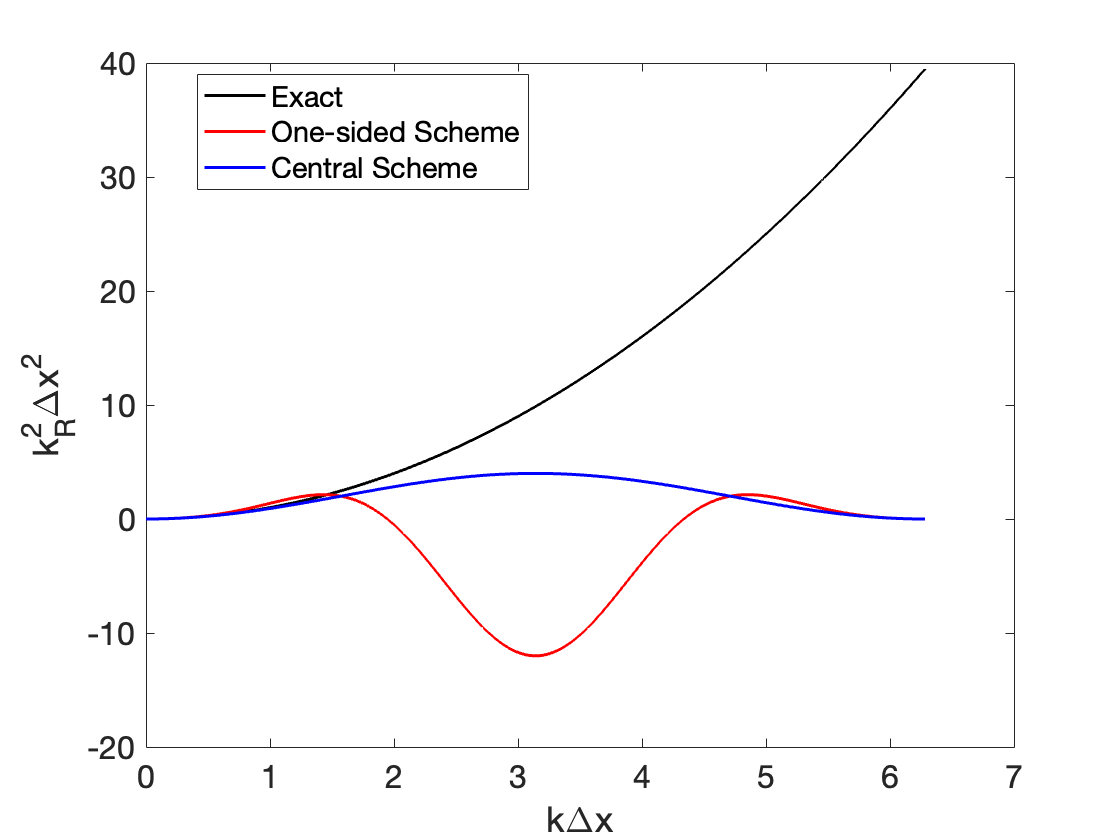
\includegraphics[width=0.5\textwidth]{p1.png}
  \caption{$e^{-\alpha k^{'2}_R t}$ plot of one-sided scheme and central scheme. }
  \label{fig1_1}
\end{figure}

For central scheme, real component of modified wavenumber is positive, which is the same as exact wavenumber. So the factor would not exceed $1$ and 
the numerical stability is ensured. But for one-sided scheme, real component of modified wavenumber could be negative, making numerical solutions grow unbounded. 
So the one-sided scheme on the diffusion equation would lead to numerical instability. 
\newpage
\section{One-Dimensional Diffusion Equation}
\subsection{a}
\subsubsection{Direct Derivation}
The time step could still be uniform, so the forward-time scheme, 
\begin{equation*}
  \frac{\partial u}{\partial t}=\frac{u_j^{n+1}-u_j^n}{\Delta t}
\end{equation*}

For non-uniform grid, 
\begin{align*}
  u_{j+1}&=u_j + \frac{\partial u}{\partial x}(x_{j+1}-x_j)+\frac{\partial^2 u}{\partial x^2}\frac{(x_{j+1}-x_j)^2}{2}\\
  u_{j-1}&=u_j + \frac{\partial u}{\partial x}(x_{j-1}-x_j)+\frac{\partial^2 u}{\partial x^2}\frac{(x_{j-1}-x_j)^2}{2}\\
  \frac{u_{j+1}}{x_{j+1}-x_j}&=\frac{u_j}{x_{j+1}-x_j}+\frac{\partial u}{\partial x}+\frac{\partial^2 u}{\partial x^2}\frac{(x_{j+1}-x_j)}{2}\\
  \frac{u_{j-1}}{x_j-x_{j-1}}&=\frac{u_j}{x_j-x_{j-1}}-\frac{\partial u}{\partial x}+\frac{\partial^2 u}{\partial x^2}\frac{(x_{j-1}-x_j)}{2}\\
  \frac{u_{j+1}}{x_{j+1}-x_j}+\frac{u_{j-1}}{x_j-x_{j-1}}&=\frac{u_j}{x_{j+1}-x_j}+\frac{u_j}{x_j-x_{j-1}}+\frac{\partial^2 u}{\partial x^2}\frac{(x_{j+1}-x_{j-1})}{2}\\
  \Rightarrow \frac{\partial^2 u}{\partial x^2}&=\frac{2}{(x_{j+1}-x_{j-1})(x_{j+1}-x_j)}u_{j+1}\\
  &-\left(\frac{2}{(x_{j+1}-x_{j-1})(x_{j+1}-x_j)}+\frac{2}{(x_{j+1}-x_{j-1})(x_j-x_{j-1})}\right)u_j+\frac{2}{(x_{j+1}-x_{j-1})(x_j-x_{j-1})}u_{j-1}\\
  &=\frac{2}{(x_{j+1}-x_{j-1})(x_{j+1}-x_j)}u_{j+1}-\frac{2}{(x_{j+1}-x_{j})(x_j-x_{j-1})}u_j+\frac{2}{(x_{j+1}-x_{j-1})(x_j-x_{j-1})}u_{j-1}
\end{align*}

Combing them for the FTCS scheme for non-uniform grid. 
\begin{align*}
  \frac{\partial u}{\partial t}&=\alpha\frac{\partial^2 u}{\partial x^2}\\
  \frac{u_j^{n+1}-u_j^n}{\Delta t}&=\frac{2\alpha}{(x_{j+1}-x_{j-1})(x_{j+1}-x_j)}u_{j+1}-\frac{2\alpha}{(x_{j+1}-x_{j})(x_j-x_{j-1})}u_j+\frac{2\alpha}{(x_{j+1}-x_{j-1})(x_j-x_{j-1})}u_{j-1}\\
  u_j^{n+1}&=u_j\\
  &+\alpha \Delta t\left(\frac{2}{(x_{j+1}-x_{j-1})(x_{j+1}-x_j)}u_{j+1}-\frac{2}{(x_{j+1}-x_{j})(x_j-x_{j-1})}u_j+\frac{2}{(x_{j+1}-x_{j-1})(x_j-x_{j-1})}u_{j-1}\right)
\end{align*}

Now considering periodic boundary conditions, $u_0=u_N$. So in practice the point $x_0$ could be seen as $x_N$. That is, the left point of $x_0$ 
could be $x_{N-1}$ and the right point of $x_{N}$ could be $x_1$. And to keep $u_0=u_N$, only one of $u_0$ and $u_N$ will be used in simulation. 
For convenience of notation, in matlab, $u_N$ is used. In that case, since $x_j=\frac{\tanh\left(5\frac{j-N/2}{N/2}\right)}{\tanh 5}$ is an odd function, 
the $dx$ is symmetric about the grid center. Therefore $x_{N+1}-x_{N}=x_1-x_0$. 
\begin{align*}
  \frac{\partial^2 u_1}{\partial x^2}&=\frac{2}{(x_{2}-x_{0})(x_{2}-x_1)}u_{2}-\frac{2}{(x_{2}-x_{1})(x_1-x_{0})}u_1+\frac{2}{(x_{2}-x_{0})(x_1-x_{0})}u_{0}\\
  &=\frac{2}{(x_{2}-x_{0})(x_{2}-x_1)}u_{2}-\frac{2}{(x_{2}-x_{1})(x_1-x_{0})}u_1+\frac{2}{(x_{2}-x_{0})(x_1-x_{0})}u_{N}\\
  \frac{\partial^2 u_N}{\partial x^2}&=\frac{2}{(x_{N+1}-x_{N-1})(x_{N+1}-x_N)}u_{N+1}-\frac{2}{(x_{N+1}-x_{N})(x_N-x_{N-1})}u_N+\frac{2}{(x_{N+1}-x_{N-1})(x_N-x_{N-1})}u_{N-1}\\
  &=\frac{2}{(x_{N+1}-x_{N-1})(x_{N+1}-x_N)}u_{1}-\frac{2}{(x_{N+1}-x_{N})(x_N-x_{N-1})}u_N+\frac{2}{(x_{N+1}-x_{N-1})(x_N-x_{N-1})}u_{N-1}\\
  x_{N+1}-x_N&=x_1-x_0\\
  x_{N+1}-x_{N-1}&=x_1-x_0+x_N-x_{N-1}=2(x_1-x_0)
\end{align*}

So the matrix form of the scheme is, 
\begin{equation*}
  \begin{bmatrix}
    u_1^{n+1}\\u_2^{n+1}\\...\\u_{N-1}^{n+1}\\u_N^{n+1}
  \end{bmatrix} = 
  I \begin{bmatrix}
    u_1\\u_2\\...\\u_{N-1}\\u_N
  \end{bmatrix} + 2\alpha \Delta t A
\end{equation*}

Matrix $A$ is shown below, 
\begin{equation*}
  \begin{bmatrix}
    -\frac{1}{(x_{2}-x_{1})(x_1-x_{0})}&\frac{1}{(x_{2}-x_{0})(x_{2}-x_1)}&...&...&\frac{1}{(x_{2}-x_{0})(x_1-x_{0})}\\
    \frac{1}{(x_{3}-x_{1})(x_2-x_{1})}&-\frac{1}{(x_{3}-x_{2})(x_2-x_{1})}&\frac{1}{(x_{3}-x_{1})(x_{3}-x_2)}&...&0\\
    ...&...&...&...&...\\
    0&...&\frac{1}{(x_{N}-x_{N-2})(x_{N-1}-x_{N-2})}&-\frac{1}{(x_{N}-x_{N-1})(x_{N-1}-x_{N-2})}&\frac{1}{(x_{N}-x_{N-2})(x_{N}-x_{N-1})}\\
    \frac{1}{2(x_1-x_0)^2}&...&...&\frac{1}{2(x_1-x_0)(x_N-x_{N-1})}&-\frac{1}{(x_1-x_0)(x_N-x_{N-1})}
  \end{bmatrix}
\end{equation*}

With $p2\_1.m$, eigenvalues of matrix $A$ are calculated numerically. 
\begin{equation*}
  \frac{\lambda_{max}}{\lambda_{min}}=\frac{7.0991359e+9}{5.4662397e-11}\approx 1.2987239e+20
\end{equation*}
\subsubsection{Coordinate Transformation}
Considering coordinate transformation, 
\begin{align*}
  \zeta &= 5\frac{j-N/2}{N/2}\\
  x&= \frac{\tanh \zeta}{\tanh 5}\\
  \Rightarrow \zeta &= \tanh ^{-1} (x \tanh 5) = g(x)
\end{align*}

With chain rule, derivatives under new coordinate system could be derived. 
\begin{align*}
  \frac{du}{dx}&= \frac{d \zeta}{dx}\frac{du}{d\zeta}=g'\frac{du}{d\zeta}\\
  \frac{d^2 u}{dx^2} &= \frac{d}{d x}\left[g'\frac{du}{d\zeta}\right]=g''\frac{du}{d\zeta}+(g')^2\frac{d^2u}{d\zeta^2}
\end{align*}

Substituting $\zeta$ and $g$ and taking $\tanh 5 = a$. 
\begin{align*}
  g' &= \frac{a}{1-a^2x^2}\\
  g''&= \frac{2a^3x}{(1-a^2x^2)^2}\\
  \frac{du}{dx}&= \frac{a}{1-a^2x^2}\frac{u_{j+1}-u_{j-1}}{2\Delta \zeta}\\
  \frac{d^2 u}{dx^2} &= \frac{2a^3x}{(1-a^2x^2)^2}\frac{u_{j+1}-u_{j-1}}{2\Delta \zeta} + \left(\frac{a}{1-a^2x^2}\right)^2 \frac{u_{j+1}-2u_j+u{j-1}}{\Delta \zeta^2}\\
  &= \frac{a^3x}{(1-a^2x^2)^2}\frac{u_{j+1}-u_{j-1}}{\Delta \zeta} + \frac{a^2}{(1-a^2x^2)^2} \frac{u_{j+1}-2u_j+u{j-1}}{\Delta \zeta^2}\\
  &= \frac{a^2}{(1-a^2x^2)^2\Delta \zeta}\left[\left(\frac{1}{\Delta \zeta}-ax\right)u_{j-1}-\frac{2}{\Delta \zeta}u_j+\left(\frac{1}{\Delta \zeta}+ax\right)u_{j+1}\right]
\end{align*}

Therefore $A$ is still a tridiagonal matirx. Sine $1-a^2x^2$ is changing with $j$, the factor of $A$ is $\frac{\alpha a^2 \Delta t}{\Delta \zeta}$. 

$\frac{1}{(1-a^2x^2)^2}\left(\frac{1}{\Delta \zeta}-ax\right)$, $-\frac{1}{(1-a^2x^2)^2}\frac{2}{\Delta \zeta}$, $\frac{1}{(1-a^2x^2)^2}\left(\frac{1}{\Delta \zeta}+ax\right)$ 
construct the three diagonals of $A$. With $p2\_2.m$, eigenvalues of matrix $A$ are calculated numerically. 
\begin{equation*}
  \frac{\lambda_{max}}{\lambda_{min}}=\frac{1.2031589e+9}{3.7371737e-11}\approx 3.2194353e+19
\end{equation*}

Therefore, for both methods, the system is stiff. 
\subsection{b}
For FTCS scheme, Explicit Euler is used for time forward. Then the stability limit of EE could be recalled. 
\begin{equation*}
  \Delta t_{max} = \frac{2}{\alpha|\lambda_{max}|}
  \Rightarrow \alpha \Delta t_{max} = \frac{2}{|\lambda_{max}|}
\end{equation*}

By $p2\_3.m$, the $\alpha \Delta t_{max}$ from the two methods are shown in Fig.~\ref{fig2_1}. 
\begin{figure}[b]
  \centering
    \begin{minipage}[t]{0.45\linewidth}
    \centering
    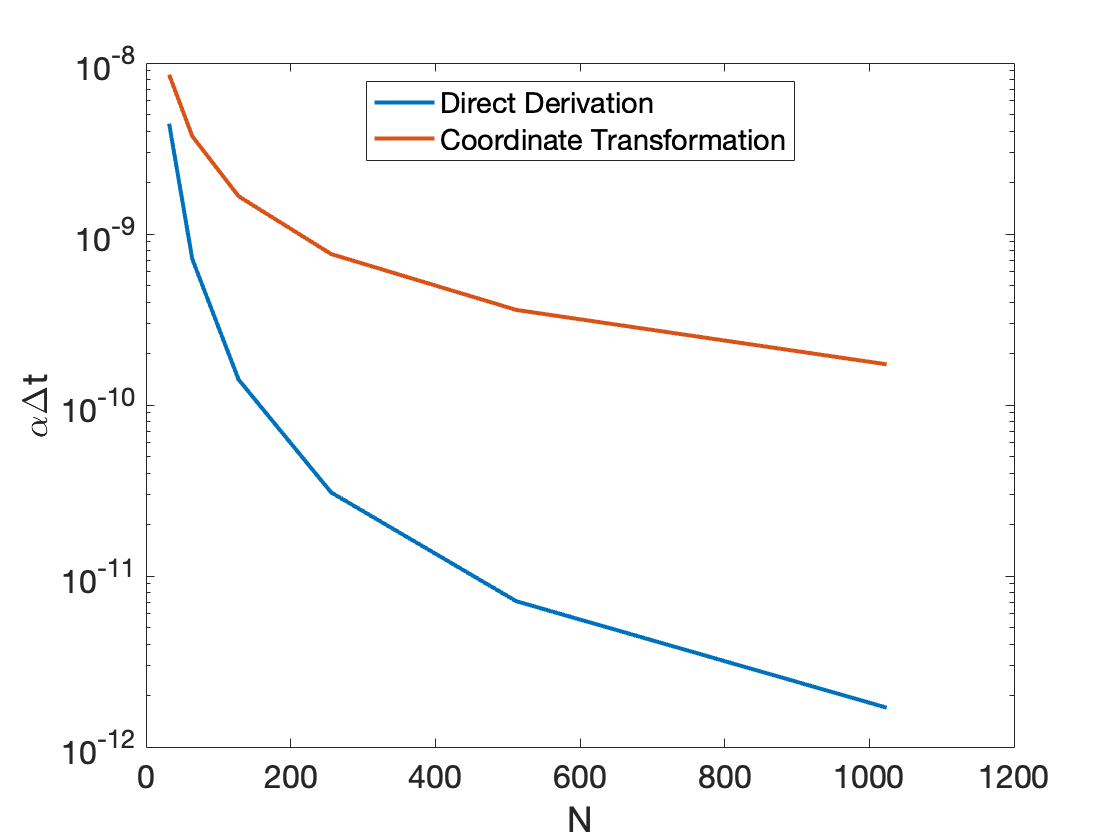
\includegraphics[width=2.3in]{p2_1.png}
    \end{minipage}
    \begin{minipage}[t]{0.45\linewidth}
    \centering
    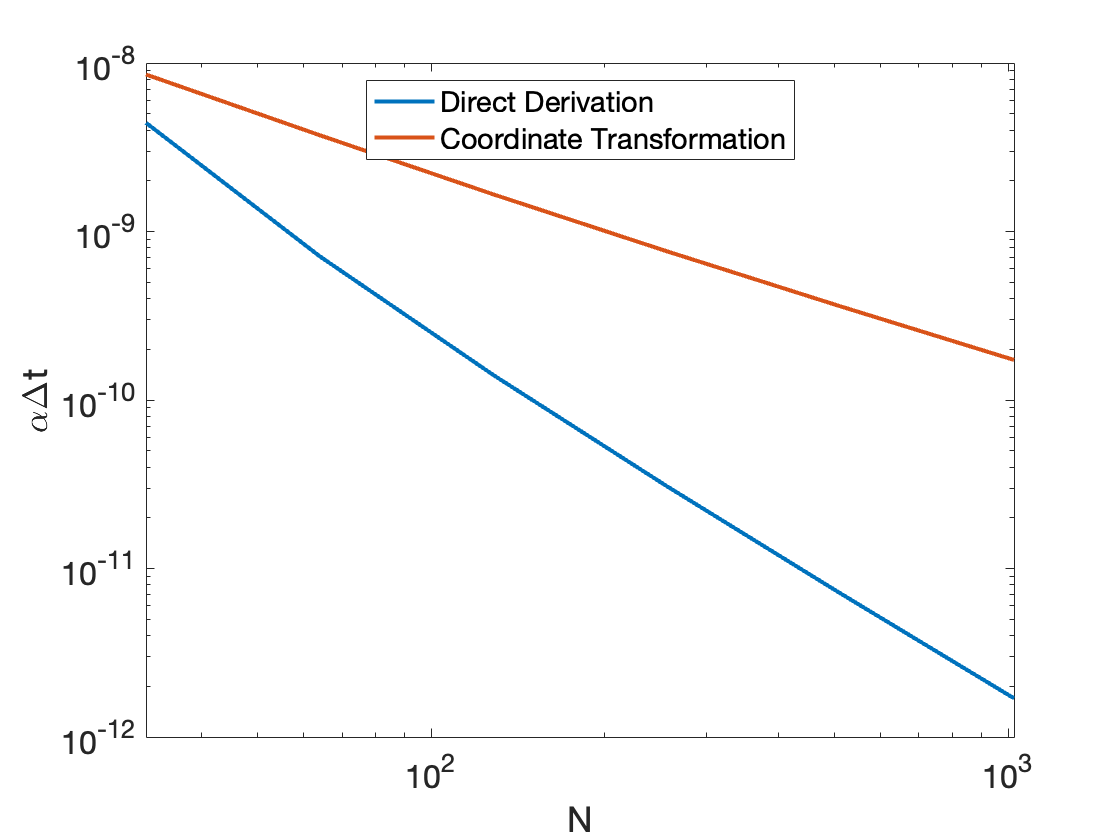
\includegraphics[width=2.3in]{p2_3.png}
    \end{minipage}
  \caption{$N$-$\alpha \Delta t_{max}$ plot of two methods. }
  \label{fig2_1}
\end{figure}

Through coordinate transformation, the required $\Delta t_{max}$ is larger than direct derivation. 
\subsection{c}
Considering the direct derivation, 
\begin{align*}
  u_j^{n+1}&=u_j\\
  &+\alpha \Delta t\left(\frac{2}{(x_{j+1}-x_{j-1})(x_{j+1}-x_j)}u_{j+1}-\frac{2}{(x_{j+1}-x_{j})(x_j-x_{j-1})}u_j+\frac{2}{(x_{j+1}-x_{j-1})(x_j-x_{j-1})}u_{j-1}\right)\\
  \sigma&=1\\
  &+\alpha \Delta t\left(\frac{2}{(x_{j+1}-x_{j-1})(x_{j+1}-x_j)}e^{ikx_{j+1}}-\frac{2}{(x_{j+1}-x_{j})(x_j-x_{j-1})}+\frac{2}{(x_{j+1}-x_{j-1})(x_j-x_{j-1})}e^{ikx_{j-1}}\right)\\
  |\sigma|&<|1+\alpha \Delta t\left(\frac{2}{2\Delta x_{min}^2}e^{ikx_{j+1}}-\frac{2}{\Delta x_{min}^2}+\frac{2}{2\Delta x_{min}^2}e^{ikx_{j-1}}\right)|\\
  |\sigma|&<|1+\frac{2\alpha \Delta t}{\Delta x_{min}^2}\left(\cos \Delta x -1\right)|\\
  \Rightarrow \alpha \Delta t &\leq \frac{\Delta x_{min}^2}{2}
\end{align*}

Considering the coordinate transformation method, 
\begin{align*}
  u_j^{n+1}&=u_j^n+ \frac{a^2\alpha \Delta t}{(1-a^2x^2)^2\Delta \zeta}\left[\left(\frac{1}{\Delta \zeta}-ax\right)u_{j-1}-\frac{2}{\Delta \zeta}u_j+\left(\frac{1}{\Delta \zeta}+ax\right)u_{j+1}\right]\\
  \sigma^{n+1}e^{ik\zeta_j}&=\sigma^ne^{ik\zeta_j}+\frac{a^2\alpha \Delta t}{(1-a^2x^2)^2\Delta \zeta}\left[\left(\frac{1}{\Delta \zeta}-ax\right)\sigma^ne^{ik\zeta_{j-1}}-\frac{2}{\Delta \zeta}\sigma^ne^{ik\zeta_j}+\left(\frac{1}{\Delta \zeta}+ax\right)\sigma^ne^{ik\zeta_{j+1}}\right]\\
  \sigma&=1+\frac{a^2\alpha \Delta t}{(1-a^2x^2)^2\Delta \zeta}\left[\left(\frac{1}{\Delta \zeta}-ax\right)e^{-ik\Delta\zeta}-\frac{2}{\Delta \zeta}+\left(\frac{1}{\Delta \zeta}+ax\right)e^{ik\Delta\zeta}\right]\\
  |\sigma|&=|1+\frac{a^2\alpha \Delta t}{(1-a^2x^2)^2\Delta \zeta}\left[\left(\frac{1}{\Delta \zeta}-ax\right)\left(\cos\Delta\zeta-i\sin\Delta\zeta\right)-\frac{2}{\Delta \zeta}+\left(\frac{1}{\Delta \zeta}+ax\right)\left(\cos\Delta\zeta+i\sin\Delta\zeta\right)\right]|\\
  |\sigma|&=|1+\frac{a^2\alpha \Delta t}{(1-a^2x^2)^2\Delta \zeta^2}\left[\left(1-ax\Delta \zeta\right)\left(\cos\Delta\zeta-i\sin\Delta\zeta\right)-2+\left(1+ax\Delta \zeta\right)\left(\cos\Delta\zeta+i\sin\Delta\zeta\right)\right]|
\end{align*}

$\Delta \zeta$ is small, so $|\sigma|$ could be approximated and simplified. 
\begin{align*}
  |\sigma|&\approx |1+\frac{a^2\alpha \Delta t}{(1-a^2x^2)^2\Delta \zeta^2}\left[\left(\cos\Delta\zeta-i\sin\Delta\zeta\right)-2+\left(\cos\Delta\zeta+i\sin\Delta\zeta\right)\right]|\\
  |\sigma|&= |1+\frac{a^2\alpha \Delta t}{(1-a^2x^2)^2\Delta \zeta^2}\left[2\cos\Delta\zeta-2\right]|
\end{align*}

Obviously when $|x|=1$, $|\sigma|$ would be the greatest. 
\begin{align*}
  |\sigma|&= |1+\frac{a^2\alpha \Delta t}{(1-a^2)^2\Delta \zeta^2}\left[2\cos\Delta\zeta-2\right]|<1\\
  -1&<1+\frac{a^2\alpha \Delta t}{(1-a^2)^2\Delta \zeta^2}\left[2\cos\Delta\zeta-2\right]<1\\
  \frac{a^2\alpha \Delta t}{(1-a^2)^2\Delta \zeta^2}&<\frac{1}{1-\cos\Delta\zeta}\leq\frac{1}{2}\\
  \alpha \Delta t &\leq \frac{(1-a^2)^2\Delta \zeta^2}{2a^2}
\end{align*}

By $p2\_4.m$, the $\alpha \Delta t_{max}$ from the four methods are shown in Fig.~\ref{fig2_2}. 
\begin{figure}[h]
  \centering
    \begin{minipage}[t]{0.45\linewidth}
    \centering
    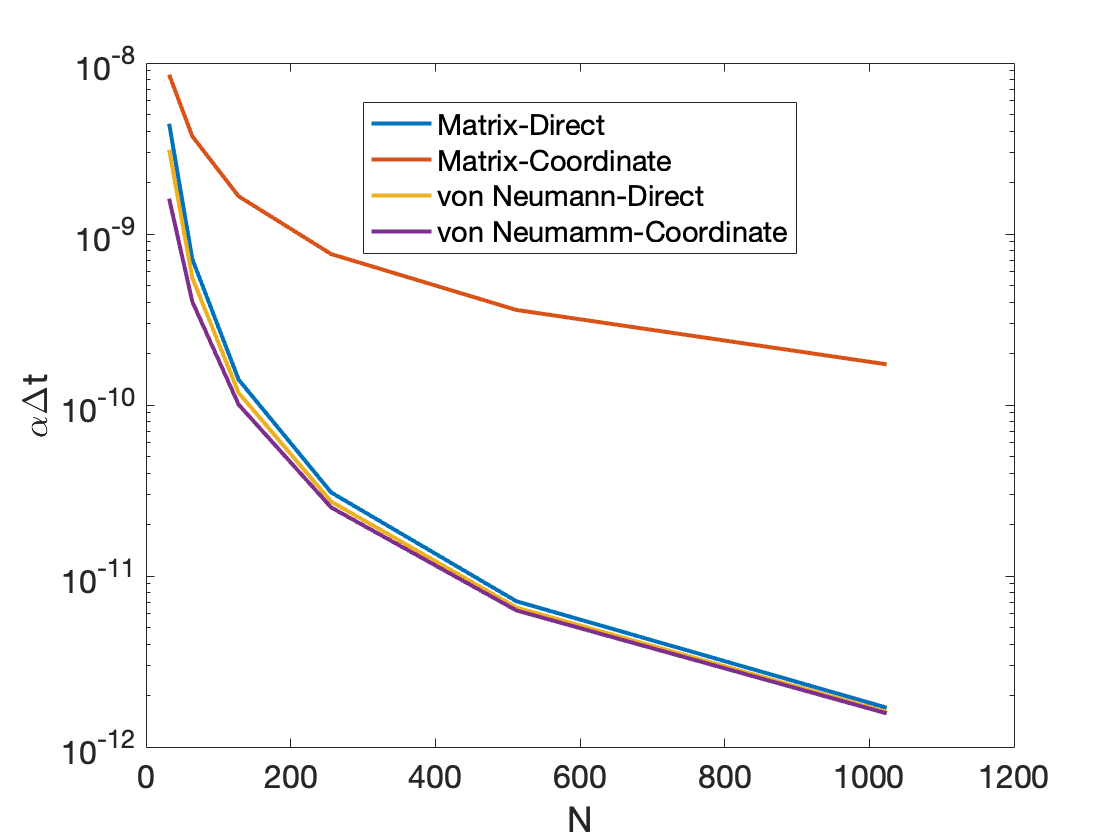
\includegraphics[width=2.3in]{p2_2.png}
    \end{minipage}
    \begin{minipage}[t]{0.45\linewidth}
    \centering
    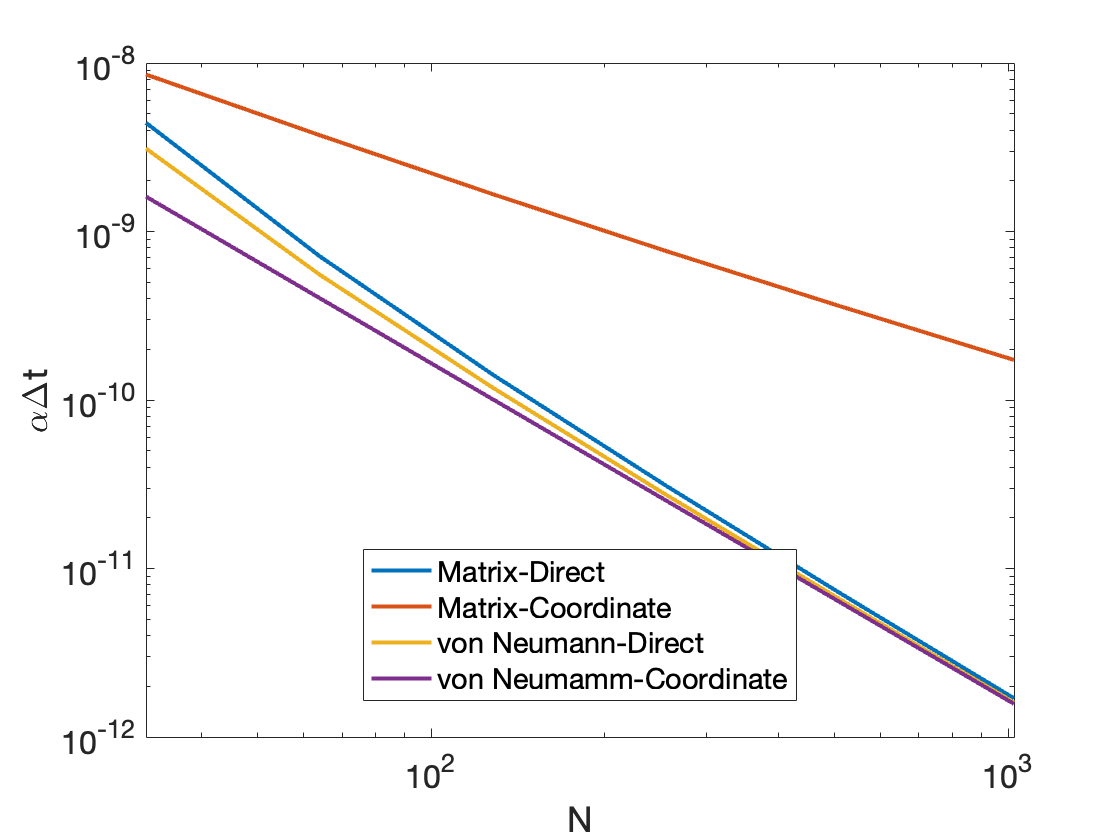
\includegraphics[width=2.3in]{p2_4.png}
    \end{minipage}
  \caption{$N$-$\alpha \Delta t_{max}$ plot of four methods. }
  \label{fig2_2}
\end{figure}

Since the idea of approximation is similar, $\alpha \Delta t_{max}$ from the two von Neumann stability are close. 
But under the amplification effects of approximation, $\alpha \Delta t_{max}$ from von Neumann stability are smaller than 
$\alpha \Delta t_{max}$ from matrix stability. And for direct derivation, the $|\lambda_{max}|$ comes from $\Delta x_{min}$ closely, 
so the $\alpha \Delta t_{max}$ from von Neumann stability are also close to $\alpha \Delta t_{max}$ from matrix stability of direct derivation, 
which is only slightly larger. 
\section{Multi-Dimensional Convection Equation}
\subsection{a}
To retain the initial energy, when there is no dissipation in the convection equation, that means the dissipation error should be eliminated. 
So modified wavenumber stability analysis is used to analyze the dissipation. Since same scheme will be used on different spatial directions, 
considering one-dimensional case is enough for modified wavenumber stability analysis. 
\begin{align*}
  u&=\psi_0 e^{ik(x-ct)}\\
  \frac{\partial u}{\partial t}&= -c\frac{\partial u}{\partial x}=-c\\
  u&=\psi_0 e^{ck'_It} e^{ik\left(x-\frac{k'_R}{k}ct\right)}
\end{align*}

The factor $e^{ck'_It}$ will lead to dissipation error. So the spatial scheme should not have imaginary component in the modified wavenumber. 
For example, central-difference scheme do not have such term. In that problem there is no other need for higher-order spatial scheme. So 
second-order central difference scheme for spatial difference is enough. 

For choice of time scheme, here is a new requirement. To retain initial energy, dissipation error is eliminated, there will be only dispersion error in 
the scheme, which means purely imaginary eigenvalues. So naturally, the time scheme chosen must has imaginary-axis stability. That is why 
Explicit Euler is unconditional unstable for convection equation. 

To compare discretization and maximum time step, von Neumann stability analysis is used based on second-order central difference scheme. Taking 
$\Delta x=\Delta y=h$. For explicit methods, 
\begin{align*}
  \frac{\partial u}{\partial t}&=-\frac{1}{2h}\left(u_{i+1,j}-u_{i-1,j}\right)-\frac{1}{h}\left(u_{i,j+1}-u_{i,j-1}\right)\\
  \Delta t &\leq \frac{2.83}{|\lambda_{max}|}=\frac{2.83}{|\frac{1}{h}i\cos\left(\frac{\pi i}{N}\right)+\frac{2}{h}i\cos\left(\frac{\pi j}{N}\right)|}
  \leq \frac{2.83 h}{3}~for~RK4\\
  (c_x+c_y)\frac{\Delta t}{h}&\leq 1\Rightarrow \Delta t\leq\frac{h}{3}~for~Lax-Wendroff
\end{align*}

From cost and $\Delta t_{max}$, RK4 will be better than Lax-Wendroff. 

For Implicit Euler, 
\begin{align*}
  \frac{u_j^{n+1}-u_j^n}{\Delta t}&=-\frac{1}{2h}\left(u^{n+1}_{i+1,j}-u^{n+1}_{i-1,j}\right)-\frac{1}{h}\left(u^{n+1}_{i,j+1}-u^{n+1}_{i,j-1}\right)\\
  u_j^n&=u_j^{n+1}+\frac{\Delta t}{2h}\left(u^{n+1}_{i+1,j}-u^{n+1}_{i-1,j}\right)+\frac{\Delta t}{h}\left(u^{n+1}_{i,j+1}-u^{n+1}_{i,j-1}\right)\\
  1&=\sigma+\frac{3\Delta t}{2h}\sigma\left(e^{ikh}-e^{-ikh}\right)\\
  1&=\sigma+\frac{3\Delta t}{h}i\sigma\sin kh\\
  \sigma&=\frac{1}{1+i\frac{3\Delta t}{h}\sin kh}
\end{align*}

Implicit Euler is unconditionally stable, but since $|\sigma|<1$, even though central difference eliminates dissipation, implicit euler will import 
extra dissipation. 

For trapizoid method, or so-called Crank-Nicolson method in diffussion equation, 
\begin{align*}
  \frac{u_j^{n+1}-u_j^n}{\Delta t}&=-\frac{1}{4h}\left(u^{n+1}_{i+1,j}-u^{n+1}_{i-1,j}\right)-\frac{1}{4h}\left(u^{n}_{i+1,j}-u^{n}_{i-1,j}\right)
  -\frac{1}{2h}\left(u^{n+1}_{i,j+1}-u^{n+1}_{i,j-1}\right)-\frac{1}{2h}\left(u^{n}_{i,j+1}-u^{n}_{i,j-1}\right)\\
  \frac{\sigma-1}{\Delta t}&=-\frac{3}{4h}\sigma\left(e^{ikh}-e^{-ikh}\right)-\frac{3}{4h}\left(e^{ikh}-e^{-ikh}\right)\\
  \sigma &= \frac{1-\frac{3\Delta t}{2h}i\sin kh}{1+\frac{3\Delta t}{2h}i\sin kh}
\end{align*}

For trapizoid, $|\sigma|=1$. So trapizoid method with central difference scheme will ont import any dissipation and it is unconditionally stable. 
In summary, central difference with trapizoid method, or Crank-Nicolson method should be the best choice. Second-order accuracy in time and space will 
not be too expensive and it will not import any dissipation. So trapizoid is better than implicit euler. 

For different schemes, than bad methods on fine grid should be faster good numerical mothods on coarse grid. Generally, better scheme brings larger 
computation cost, compared to the tolerence it brings. So when the two schemes both meet the requirements, scheme with not such high order of accuracy 
will be more practical to implement. 
\subsection{b}
In that problem, one cycle time could be defined as $\frac{2\pi}{c_{min}}=2\pi$. So ten cycles actually requires total time of $20\pi$. 
And 2-D implicit method is expensive and hard to implement, firstly RK4 is used in this problem. With $p3\_1.m$, the energy reduces to less than $99\%$ quickly. 
So explicit scheme also imports dissipation. 

Therefore the trapizoid method is the only choice to retain such initial energy for such a long cycle time. In that case, 
the solution after ten cycles should be very close to the initial condition. The scheme is implemented with $p3\_2.m$. Since it is unconditionally stable, 
the time step could be not so small. Considering the huge cost for solving huge matrices, the time step is firstly taken $0.05$. Then I changed it to 
$0.01$. 

To implement such method with 2-D dimension, I took a cubersome methed. The 2-D $u_{ij}$ is streched to a one dimensional vector, from a $512\times 512$ matriix 
to a $512^2$ vector. Then the coefficient matrix becomes $512^2\times 512^2$ and is something like penta-diagonal matrix with some modification because of 
periodic conditions. 
\begin{align*}
  \frac{u_j^{n+1}-u_j^n}{\Delta t}=-\frac{1}{4h}\left(u^{n+1}_{i+1,j}-u^{n+1}_{i-1,j}\right)-\frac{1}{4h}\left(u^{n}_{i+1,j}-u^{n}_{i-1,j}\right)
  -\frac{1}{2h}\left(u^{n+1}_{i,j+1}-u^{n+1}_{i,j-1}\right)-\frac{1}{2h}\left(u^{n}_{i,j+1}-u^{n}_{i,j-1}\right)&\\
  u_j^{n+1}+\frac{1}{4h}\left(u^{n+1}_{i+1,j}-u^{n+1}_{i-1,j}\right)+\frac{1}{2h}\left(u^{n+1}_{i,j+1}-u^{n+1}_{i,j-1}\right)=
  u_j^n-\frac{1}{4h}\left(u^{n}_{i+1,j}-u^{n}_{i-1,j}\right)-\frac{1}{2h}\left(u^{n}_{i,j+1}-u^{n}_{i,j-1}\right)&\\
  \Rightarrow A u^{n+1} = B u^n&
\end{align*}

$A$ and $B$ are both matrices mentioned above, something like penta-diagonal matrix with some modification because of periodic conditions. 
After those are established, simulation could be processed by time steps. From $p3\_2.m$, the code took $4073$ seconds for $\Delta t=0.05$ and $14371$ second for $\Delta t = 0.01$. 
Both of them  retained $99.99999999999999\%$ of initial energy. The output of Matlab is shown in Fig.~\ref{fig3_1}. 
\begin{figure}[h]
  \centering
    \begin{minipage}[t]{0.6\linewidth}
    \centering
    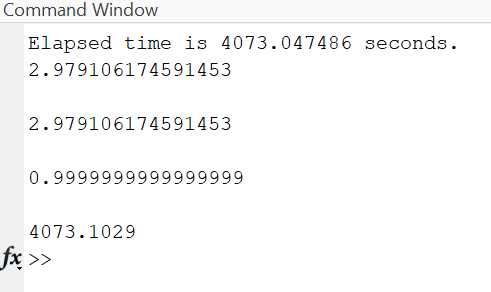
\includegraphics[width=3in]{p3_1.png}
    \end{minipage}
    \begin{minipage}[t]{0.6\linewidth}
    \centering
    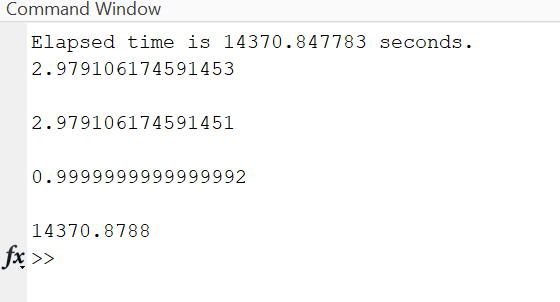
\includegraphics[width=3in]{p3_2.png}
    \end{minipage}
  \caption{Matlab output of trapizoid method with central difference scheme. }
  \label{fig3_1}
\end{figure}
\end{document}